
%(BEGIN_QUESTION)
% Copyright 2007, Tony R. Kuphaldt, released under the Creative Commons Attribution License (v 1.0)
% This means you may do almost anything with this work of mine, so long as you give me proper credit

Suppose an empty test vessel of fixed volume is immersed in an ice-water mixture and allowed to stabilize at that temperature, with a bleed valve left open to equalize the vessel's air pressure with ambient (atmospheric) pressure at sea level:

$$\includegraphics[width=15.5cm]{i02970x01.eps}$$

Once stabilized, the valve is shut off and the vessel is taken out of the ice-water bath, then left to stabilize at room temperature (70$^{o}$ F).  Calculate the pressure built up inside the vessel resulting from the increased temperature, in units of inches water column ("W.C.).

\underbar{file i02970}
%(END_QUESTION)





%(BEGIN_ANSWER)

Assuming volume ($V$), molecular gas quantity ($n$), and the Gas Constant ($R$) never change, the Ideal Gas Law may be reduced as follows:

$$P_1V = nRT_1$$

$$P_2V = nRT_2$$

$${P_1V \over P_2V} = {nRT_1 \over nRT_2}$$

$${P_1 \over P_2} = {T_1 \over T_2}$$

$$P_2 = P_1 {T_2 \over T_1}$$

\vskip 10pt

$P_1$ at 0$^{o}$ C = 1 atm = 14.7 PSIA

$T_1$ at 0$^{o}$ C = 273.15 K

$T_2$ at 70$^{o}$ F = 21.11$^{o}$ C = 294.26 K

\vskip 10pt

$$P_2 = 14.7 \hbox{ PSIA} \left({294.26 \hbox{ K} \over 273.15 \hbox{ K}}\right)$$

\vskip 10pt

$P_2$ = 15.84 PSIA = 1.136 PSIG = 31.5 "W.C.

%(END_ANSWER)





%(BEGIN_NOTES)


%INDEX% Physics, static fluids: ideal gas law

%(END_NOTES)


